\documentclass[tikz]{standalone}
\usepackage{times}
\usepackage{bm}
\begin{document}
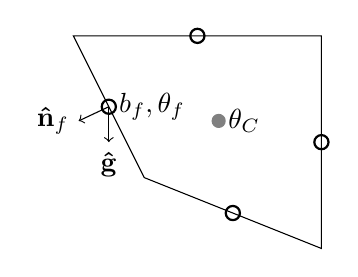
\begin{tikzpicture}[
  scale=0.45,
  cpnt/.style={fill=gray}
]

\draw (2,3) -- (0,7) -- (7,7) -- (7,1) -- (2,3);

\path [cpnt] (4.1,4.6) circle [radius=0.2] node [right] {$\theta_C$};

\draw [thick] (7,4) circle [radius=0.2];
\draw [thick] (4.5,2) circle [radius=0.2];
\draw [thick] (3.5,7) circle [radius=0.2];
\draw [thick] (1,5) circle [radius=0.2] node [right] {$b_f, \theta_f$};

\draw [->] (1,5) -- (0.15,4.6) node [left] {$\mathbf{\hat{n}}_f$};
\draw [->] (1,5) -- (1,4) node [below] {$\mathbf{\hat{g}}$};

\end{tikzpicture}
\end{document}
